\documentclass[11pt]{article}
\usepackage[utf8]{inputenc}
\usepackage[T1]{fontenc}
\usepackage{amsmath,amssymb}
\usepackage{booktabs}
\usepackage{graphicx}
\usepackage{geometry}
\geometry{margin=1in}
\usepackage{authblk}
\usepackage[hidelinks]{hyperref}
\usepackage{xurl}
\usepackage{caption}
\usepackage{xcolor}
\usepackage{titlesec}
\usepackage{tikz}
\usepackage[section]{placeins}
\usetikzlibrary{positioning,arrows.meta}
\definecolor{navy}{HTML}{1A3A5C}
\definecolor{accent}{HTML}{2563EB}
\titleformat{\section}{\normalfont\Large\bfseries\color{navy}}{\thesection}{1em}{}
\titleformat{\subsection}{\normalfont\large\bfseries\color{accent}}{\thesubsection}{1em}{}
\graphicspath{{figures/}}
\setlength{\emergencystretch}{2em}

\newcommand{\zindiuser}{\texttt{craigouma}}
\newcommand{\gap}{\operatorname{gap}}

\title{\textbf{Rebuilding the Coverage Gap Score from Public Reference
Data, and Unnamed Local Roads on Tribal Reservations: Methodology for the
Bias Bounty Mapping Equity Challenge}}

\author[1]{Craig Carlos Ouma\thanks{%
Correspondence: \texttt{craigcarlos95@gmail.com}. Zindi: \zindiuser. Final
submissions: S24 (\texttt{EC3xBxjr}) and S19 (\texttt{Ekx9Rx3y}). Code:
private repository, released to Zindi reviewers on request.}}
\affil[1]{Independent Researcher}
\date{\today}

\begin{document}
\maketitle

\begin{abstract}
\noindent
The challenge asks for a coverage gap score per Census tract that compares
Overture Maps release 2026-08-19.0 with reference data for roads, buildings
and points of interest across 9,794 tracts in five hazard regions of the
western and southern United States. No labels are provided, so every
submission is an estimate of a deterministic formula applied to reference
layers that the organisers removed from the challenge bucket on 25 September
2026. Over sixteen submissions an estimation approach built only from the
challenge package brought the public RMSE from 0.1072 for the all-zero file to
0.0745. After Zindi staff confirmed on 27 October that the public versions of
those layers could be used, the pipeline rebuilt the reference side of each component from those sources and
reached 0.02996 (submission S19), then 0.02380 (S24) once ZIP establishment
counts were apportioned to tracts by HUD business-address ratios. The rebuilt
transport component reproduces
the organisers' published undefined rates to within one percentage point in
all four documented regions, and their published spread of road length ratios
(0.71 to 1.59) once road length on shared tract boundaries is counted once.
The submissions that tested alternative building, EMS, school and
establishment references show where the remaining error sits.
For the Best Bias Discovery track, this paper reports that on federally
recognised reservations the share of local street length with no name in
Overture is 9.5 percentage points higher than on non-tribal tracts of the same
region and rurality (95\,\% county bootstrap interval 3.5 to 14.7), rising to
27.6 points on the Osage Reservation, while highways there are named at the
same rate as elsewhere. The scorecard cannot see this because it measures
length and counts. Emergency dispatch and evacuation messaging depend on the
names.
\end{abstract}

\section{Introduction}
\label{sec:intro}

The Bias Bounty Mapping Equity Challenge, run on Zindi by Humane Intelligence
with Reliabl and Radiant Earth, asks how complete open map data is in places
exposed to heat, drought and wildfire, and whether the gaps fall unevenly
across rural, tribal and socially vulnerable communities. Each scored tract
receives a composite score $y \in [0, 1]$, with 0 meaning Overture matches the
reference and 1 meaning Overture has nothing where the reference has
something. Ranking is by root mean squared error (RMSE) on $y$, with about
30\,\% of tracts on the public leaderboard and 70\,\% on the private one.

The score is a formula. It is the mean of up to three components (transport,
building, points of interest), each comparing an Overture quantity with a
reference quantity in the same tract. The Overture side is in the challenge
package. The reference side was removed from the package on 25 September 2026
(TIGER/Line roads, Microsoft building footprints, HIFLD and USGS facilities,
and Census Business Patterns establishments), so the task becomes the
estimation of a formula whose inputs are partly hidden.

This paper documents the pipeline that produced the final submissions, how
each component was computed, the edge cases, the alternatives that were tried
and why each was kept or dropped, and a bias pattern that the automated Bias
Scorecard cannot detect. Section~\ref{sec:data} lists the data.
Section~\ref{sec:pipeline} describes the pipeline.
Section~\ref{sec:components} defines each component and how it was computed.
Section~\ref{sec:edge} covers the edge cases. Section~\ref{sec:history} gives
the full submission history with the evidence each one produced.
Section~\ref{sec:scorecard} reflects on the scorecard and
Section~\ref{sec:bias} presents the bias discovery.

All submissions were made by Zindi user \zindiuser{}, entering solo.
The two submissions selected for private scoring are S24 (public RMSE
0.023796, Zindi ID \texttt{EC3xBxjr}) and S19 (0.029961, \texttt{Ekx9Rx3y}),
described in Section~\ref{sec:final}; the
others referred to in this paper are listed in Table~\ref{tab:history}.

\section{Data}
\label{sec:data}

\subsection{Challenge package}

All challenge data were read from the challenge's public Source Cooperative
bucket \cite{bucket} on 25 October 2026. The bucket held 327 objects; 172 files (4,615,029,100 bytes)
were synced to Kaggle, every byte count was checked against the listing, and
all matched on the first attempt. No file named for a coverage gap, TIGER,
Microsoft, HIFLD or Census Business Patterns existed anywhere in the bucket.

The pipeline uses the six Overture layers of release 2026-08-19.0 per region
(buildings, roads, unfiltered roads, rail, infrastructure, places), the ACS
2020 to 2024 housing unit counts per tract, the tract polygons and the strata
tables (Census tract table, CDC SVI 2022, Climate Vulnerability Index, RUCA
2020, RUCC 2023, tribal overlap, and the drought, heat and wildfire tables).
GEOID is kept as 11-character text in every read; an integer cast drops the
leading zero of Arizona's state code and silently breaks every Maricopa join.
Region membership comes from the \texttt{region} column of the sample
submission, which places tract \texttt{35023970000} (Hidalgo County, New
Mexico) in the Maricopa region.

Two uses of the package should be disclosed. ACS housing units, which the
organisers describe as a sanity check outside the building ratio, were used
as a feature in the estimation phase (S02 to S16). Overture's own
\texttt{sources[].dataset} attribute, which records whether a footprint came
from OpenStreetMap or a machine-learned product, was used in the same phase.
Neither enters the final submissions.

\subsection{Public reference sources}

On 27 October 2026 Zindi staff confirmed that the public versions of the
removed layers (TIGER/Line roads, Microsoft footprints, HIFLD facilities and
Census Business Patterns) could be used. Facility counts were taken from the
USGS National Map structures, which the challenge page names as the facility
reference and which is the source of the HIFLD fire station layer. The pipeline then
downloaded the sources in Table~\ref{tab:sources} directly from their
publishers inside Kaggle kernels. The one exception is the HUD USPS ZIP-TRACT
crosswalk \cite{hud}, which HUD now serves only through a token API. Its
archived copy on DataLumos (project 219325, version V2) was downloaded on 29
October 2026, the Q4 2024 ZIP-TRACT file was converted from xlsx to parquet
with ZIP and tract codes kept as text (\texttt{scripts/hud\_dataset.py}), and
the result was published as a private Kaggle dataset read by stage 07. No
earlier version of the challenge bucket,
no old challenge zip and no third-party mirror of the removed layers was
used. Organiser score files of any kind were never opened; a file guard
rejects any path containing \texttt{coverage-gap} or
\texttt{coverage\_gap} regardless of other permissions, and a unit test fails
if any reader bypasses it.

\begin{table}[htbp]
\centering
\small
\caption{Reference sources rebuilt from their publishers. ``Final'' marks the
sources used by the selected submissions S24 and S19.}
\label{tab:sources}
\resizebox{\textwidth}{!}{%
\begin{tabular}{llll}
\toprule
Source & Vintage & Used for & Final \\
\midrule
Census TIGER/Line primary and secondary roads (S1100, S1200) & 2025 & transport reference & S24, S19 \\
USGS National Map structures, fire stations (FCODE 74026) & 2026 & fire reference & S24, S19 \\
USGS National Map structures, schools (FCODE 73002 to 73005) & 2026 & school reference & S24, S19 \\
Census ZIP Code Business Patterns, establishments per ZIP & 2023 & establishments reference & S24 \\
HUD USPS ZIP-TRACT crosswalk, business-address ratios & Q4 2024 & apportioning ZIP counts & S24 \\
Census 2020 ZCTA to tract relationship file & 2020 & apportioning ZIP counts (S20) & no \\
USGS National Map structures, ambulance services (FCODE 74034) & 2026 & EMS reference (S21) & no \\
Microsoft US Building Footprints & v2 & building reference (S18) & no \\
HIFLD Open archive: fire and EMS stations, public and private schools & 2025 & S22 & no \\
\bottomrule
\end{tabular}}
\end{table}

TIGER/Line is distributed in NAD83 longitude and latitude and the tract
polygons, built from the same TIGER edges, are labelled CRS84. The pipeline
relabels TIGER as CRS84 without a transform, which keeps road and tract
boundary vertices identical; NAD83 and WGS84 differ by under two metres in
the contiguous United States.

\section{Pipeline}
\label{sec:pipeline}

Every step that reads challenge data or fits anything runs as a private
Kaggle script kernel; the laptop is used only for editing, unit tests on
synthetic fixtures and orchestration through the Kaggle command line. Code
reaches Kaggle as a private dataset built from a clean git commit, and each
kernel stops if the commit hash in the dataset differs from the one it was
rendered with. Figure~\ref{fig:pipeline} shows the stages and
Table~\ref{tab:stages} their measured cost.

\begin{figure}[htbp]
\centering
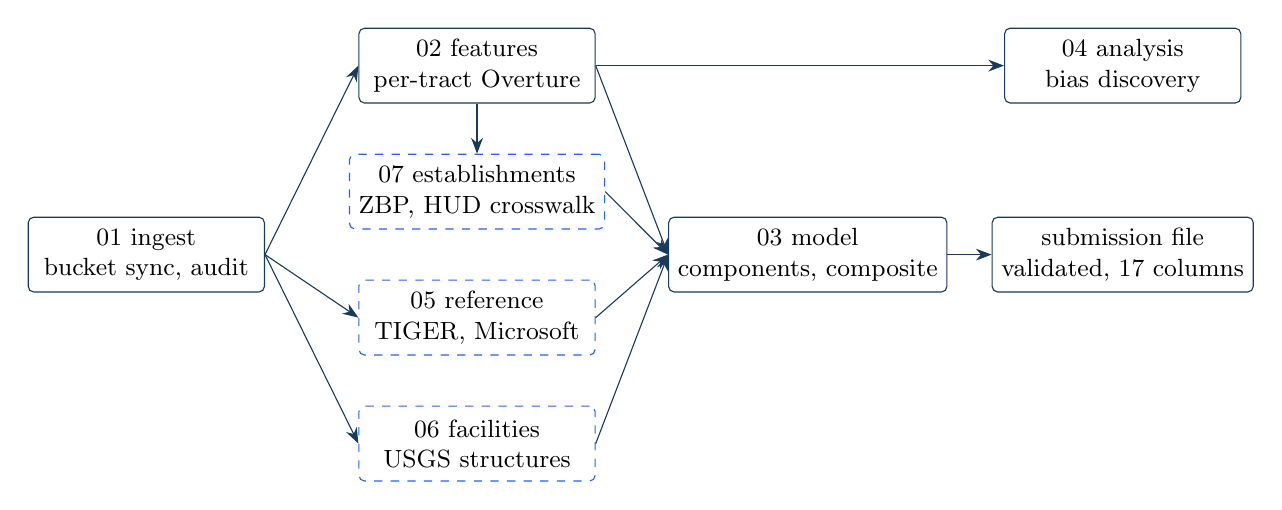
\begin{tikzpicture}[
  box/.style={draw=navy, rounded corners=2pt, align=center, font=\small,
              minimum width=3.0cm, minimum height=0.95cm},
  ext/.style={box, draw=accent, dashed},
  arr/.style={-{Stealth[length=2mm]}, draw=navy}]
\node[box] (feat) at (4.2, 2.4) {02 features\\per-tract Overture};
\node[ext] (est) at (4.2, 0.8) {07 establishments\\ZBP, HUD crosswalk};
\node[ext] (ref) at (4.2, -0.8) {05 reference\\TIGER, Microsoft};
\node[ext] (fac) at (4.2, -2.4) {06 facilities\\USGS structures};
\node[box] (ingest) at (0, 0) {01 ingest\\bucket sync, audit};
\node[box] (model) at (8.4, 0) {03 model\\components, composite};
\node[box] (val) at (12.4, 0) {submission file\\validated, 17 columns};
\node[box] (ana) at (12.4, 2.4) {04 analysis\\bias discovery};
\foreach \n in {feat, ref, fac} \draw[arr] (ingest.east) -- (\n.west);
\draw[arr] (feat) -- (est);
\foreach \n in {feat, est, ref, fac} \draw[arr] (\n.east) -- (model.west);
\draw[arr] (model) -- (val);
\draw[arr] (feat.east) -- (ana.west);
\end{tikzpicture}
\caption{Kaggle stages. Solid boxes use the challenge package only; dashed
boxes download public reference sources. Stage 08 (HIFLD archive) and stage
09 (TIGER boundary lengths) are diagnostics outside the final path.}
\label{fig:pipeline}
\end{figure}

\begin{table}[htbp]
\centering
\small
\caption{Stage cost on Kaggle CPU sessions (4 cores, 32.9\,GB RAM), from the
runs that fed the final submissions and the bias analysis. Wall time includes
queueing.}
\label{tab:stages}
\begin{tabular}{llrr}
\toprule
Stage & Run & Wall (min) & Peak RSS (GB) \\
\midrule
01 ingest & 20261025-1434-01\_ingest-398b1ba & 5.4 & 1.39 \\
02 features & 20261026-1136-02\_features-c1f6404 & 27.9 & 6.99 \\
05 reference & 20261027-2145-05\_reference-0add93b & 33.9 & 3.55 \\
06 facilities & 20261028-0024-06\_facilities-8d8b042 & 8.7 & 0.49 \\
07 establishments & 20261030-0946-07\_establishments-decc7f9 & 1.2 & 0.22 \\
03 model (S24) & 20261030-0947-03\_model-30d804e & 1.4 & 0.55 \\
03 model (S19) & 20261028-0947-03\_model-672866c & 3.6 & 0.60 \\
04 analysis & 20261030-1019-04\_analysis-8a838bb & 24.3 & 0.80 \\
\bottomrule
\end{tabular}
\end{table}

Spatial work uses DuckDB 1.5.4 with its spatial extension. Two of its
behaviours fail silently and are guarded in code and tests: transforming from
EPSG:4326 without \texttt{always\_xy} returns infinite coordinates, and
\texttt{ST\_Length\_Spheroid} on longitude and latitude order returns NaN, so
every length passes through a helper that flips coordinates, asserts a finite
result and is tested against \texttt{pyproj.Geod} to within 0.1\,\%. Lengths
are geodesic metres of each line clipped to the tract polygon.

\section{Components}
\label{sec:components}

\subsection{Score definition}

For an Overture quantity $O$ and a reference quantity $R$ in the same tract,
\begin{equation}
\gap(O, R) = \max\!\left(0,\; 1 - \frac{O}{R}\right), \qquad
\text{defined only when } R > 0.
\label{eq:gap}
\end{equation}
The composite is the mean of the defined components among transport $T$,
building $B$ and points of interest $P$,
\begin{equation}
y = \frac{\sum_{c \in \{T, B, P\}} \delta_c\, c}{\sum_{c} \delta_c},
\label{eq:composite}
\end{equation}
where $\delta_c$ is 1 when component $c$ is defined. $P$ is the mean of its
defined halves, a facilities half $F$ and an establishments half $E$, and $F$
is the mean of the defined per-type gaps for fire stations, EMS stations and
schools. Tracts with every component undefined were removed from the scored
list by the organisers, so every scored tract has at least one defined
component. An undefined component is written as 0 with its flag false.

\subsection{Transport}

$O$ is the length of Overture road segments of class motorway, trunk, primary
or secondary, clipped to the tract. $R$ is the length of TIGER/Line 2025
roads with MTFCC S1100 or S1200, clipped the same way. A TIGER road that runs
along a tract boundary intersects both neighbouring tracts and is counted in
full in each, as a clipped computation would count it. $T$ is undefined where
the tract holds no S1100 or S1200 length.

Two published facts check this rebuild without the leaderboard
(Table~\ref{tab:transport}). The share of tracts with an undefined component
was published per region; building and POI are almost never undefined, so it
should match the share with no TIGER length, and it does to within one
percentage point in all four regions. The organisers also published that the
ratio of Overture to TIGER length ranges from 0.71 to 1.59 across the four
regions. Summing clipped per-tract lengths gives 0.64 to 1.29. Counting the
TIGER length within 0.1\,m of a tract boundary a single time gives
0.73 for Eastern Oklahoma and 1.58 for South-Central Texas, the two ends of
the published range. The organisers' region totals therefore count each road
once while their per-tract values count boundary roads in both tracts, which
is the rule used here.

\begin{table}[htbp]
\centering
\small
\caption{Transport checks against published values. Undefined: share of
scored tracts with no TIGER S1100 or S1200 length. Ratio: Overture
named-class length over TIGER length, summed over the region, with boundary
TIGER length counted once.}
\label{tab:transport}
\begin{tabular}{lrrrr}
\toprule
Region & Undefined & Published & Ratio & Mean $T$ where defined \\
\midrule
Eastern Oklahoma & 0.212 & 0.21 & 0.731 & 0.355 \\
Northern California & 0.369 & 0.37 & 1.248 & 0.162 \\
South-Central Texas & 0.284 & 0.28 & 1.581 & 0.123 \\
Maricopa & 0.546 & 0.55 & 1.314 & 0.165 \\
Eastern Washington & 0.248 & n/a & 0.965 & 0.199 \\
\bottomrule
\end{tabular}
\end{table}

\subsection{Building}

$O$ is the count of Overture footprints whose centroid falls in the tract and
$R$ the Microsoft footprint count. The public Microsoft US Building Footprints
v2 release was rebuilt per tract (S18); it gives a mean $B$ of 0.003 and
raised the public RMSE from 0.0491 to 0.0546, so the organisers' footprint
release differs from the public file in ways that matter at tract level. The
final submissions therefore set $B = 0$ wherever Overture has footprints, and
$B = 1$ where it has none and the tract is still expected to hold structures
(Section~\ref{sec:edge}). $B$ is defined wherever Overture has footprints or
ACS reports housing units. The level of $B$ is the one leaderboard-tuned
scalar in S19: a constant baseline gap tested at 0.01 and 0.05 (S13), with 0
chosen.

\subsection{Points of interest}

The organisers' bucket README states how Overture places are matched:
\texttt{categories.primary} equal to \texttt{fire\_department} for fire
stations, \texttt{ambulance\_and\_ems\_services} for EMS, and
\texttt{elementary\_school}, \texttt{middle\_school}, \texttt{high\_school},
\texttt{school}, \texttt{private\_school} or \texttt{public\_school} for
schools. Each per-type gap applies Equation~\ref{eq:gap} to the Overture
count and the reference count, and is undefined where the tract holds no
reference facility of that type.

\paragraph{Facilities half.} The reference counts are USGS National Map
structure points in the tract: FCODE 74026 for fire stations and 73002 to
73005 for schools. The README states that EMS is close to one to one with its
reference and rarely binds, and that fire stations carry the facility half.
Adding EMS against USGS ambulance services (74034) made the public RMSE worse
(S21), and a line search between S19 and S21 put the best mix at 7\,\% of the
EMS change, so EMS is left out of the facility mean. Replacing USGS schools
with the HIFLD public and private school layers (S22) carried no signal
(best mix 0.2\,\%).

\paragraph{Establishments half.} The reference is Census Business Patterns
establishments. No tract-level count exists, so the organisers must have
apportioned county or ZIP counts to tracts, and their method is undocumented.
Places in Overture outnumber ZIP Business Patterns establishments by 2.0 to
2.2 to 1 in every region, so $E$ is 0 in almost every tract under any
apportionment. S19 sets $E = 0$ where the tract has residents. S20 apportions
ZIP Business Patterns 2023 counts to tracts through the 2020 ZCTA to tract
relationship file, weighting each tract's share of a ZCTA by its Overture
place count as a stand-in for business addresses, which makes $E$ positive in
1.4\,\% of tracts. A line search between S19 and S20 put the best mix at
24\,\% of the S20 change: some establishment gaps exist, placed differently
from this apportionment.

The standard tool for moving ZIP-level business counts to tracts is the HUD
USPS ZIP-TRACT crosswalk, which gives for each ZIP the share of its business
addresses (\texttt{BUS\_RATIO}) and residential addresses
(\texttt{RES\_RATIO}) in each tract. A competitor's public repository,
posted to the challenge discussion, lists the organisers' establishment
reference columns as \texttt{cbp\_estab} and \texttt{cbp\_estab\_res}, which
match these two ratios; no file from that repository was used. S24 therefore
sets the reference to ZIP Business Patterns 2023 establishments times
\texttt{BUS\_RATIO} from the Q4 2024 crosswalk, summed over the ZIPs that
reach each tract, compares it with all Overture places in the tract, and
leaves $E$ undefined where the result is 0. $E$ becomes positive in 2.4\,\%
of tracts and 253 tracts change. The public RMSE fell from 0.0300 to 0.0238,
and the line search along S19 to S24 gave $t^\ast = 1.17$, so the change is
right in full. Offline checks of the 2023 crosswalk quarters, ZBP 2022, the
residential and total ratios, and scale factors from 0.9 to 1.3 found no
variant clearly better than S24.

\subsection{Composite and definedness}

With every component rebuilt from counts and lengths, definedness follows
directly from the reference counts, and the composite in Equation~\ref{eq:composite} is
computed directly. The estimation phase (S02 to S16) instead drew 2,000 Monte
Carlo samples per tract of each component's definedness and value, dropped
draws with all three undefined to respect the conditioning on scored tracts,
and averaged the composite over the remaining draws. That code remains in the
pipeline and reduces to the direct computation when every definedness
probability is 0 or 1.

\section{Edge cases}
\label{sec:edge}

\paragraph{Zero-population tracts.} Population enters no formula. In S24, $E$
is defined wherever the apportioned establishment count is positive, which
holds in 22 of the 27 scored tracts without residents (airports, parks,
industrial land); its gap is 0 in all of them because Overture holds more
places than the apportioned count. S19 leaves $E$ undefined in these tracts.
The facility gaps are unaffected because they depend on facility points,
which can exist in a tract without residents.

\paragraph{Water-dominated tracts.} Seven Texas water tracts (codes 99xx) were
dropped from the scored list by the organisers. Two remain,
\texttt{48039990000} (Brazoria County) and \texttt{48057990000} (Calhoun
County). Neither has residents, a TIGER primary or secondary road, a USGS
fire station or school, an Overture place or an Overture footprint. The
public Microsoft file holds five footprints in the first, likely offshore
structures, and none in the second. Because a scored tract must have a
defined component, the building component is the only one that can be
defined, and with no Overture footprints its gap is 1. Both are written with $B = 1$ and a
composite of 1.

\paragraph{Tracts with no Overture data in a layer.} The Overture count or
length is 0, so the gap is 1 wherever the reference is positive and the
component is undefined where it is not. No imputation is applied to the
Overture side.

\paragraph{Cross-border tracts.} The New Mexico tract \texttt{35023970000}
belongs to the Maricopa region and the Oklahoma border tracts
\texttt{40013795900} and \texttt{40085094200} to Eastern Oklahoma. TIGER and
USGS files were downloaded for every state that holds a scored tract (Arizona,
New Mexico, California, Oklahoma, Texas, Washington), so these tracts are
treated like any other.

\paragraph{Eastern Washington.} The 415 Eastern Washington tracts appear in
the sample submission but not in the organisers' published rates. They are
processed with the same method; with rebuilt references no parameter needs
to be borrowed from other regions.

\section{Submission history}
\label{sec:history}

Every submission was registered before upload with a hypothesis, the change
against the current best and the expected direction. Table~\ref{tab:history}
lists them and Figure~\ref{fig:history} plots the scores.

\begin{figure}[htbp]
\centering
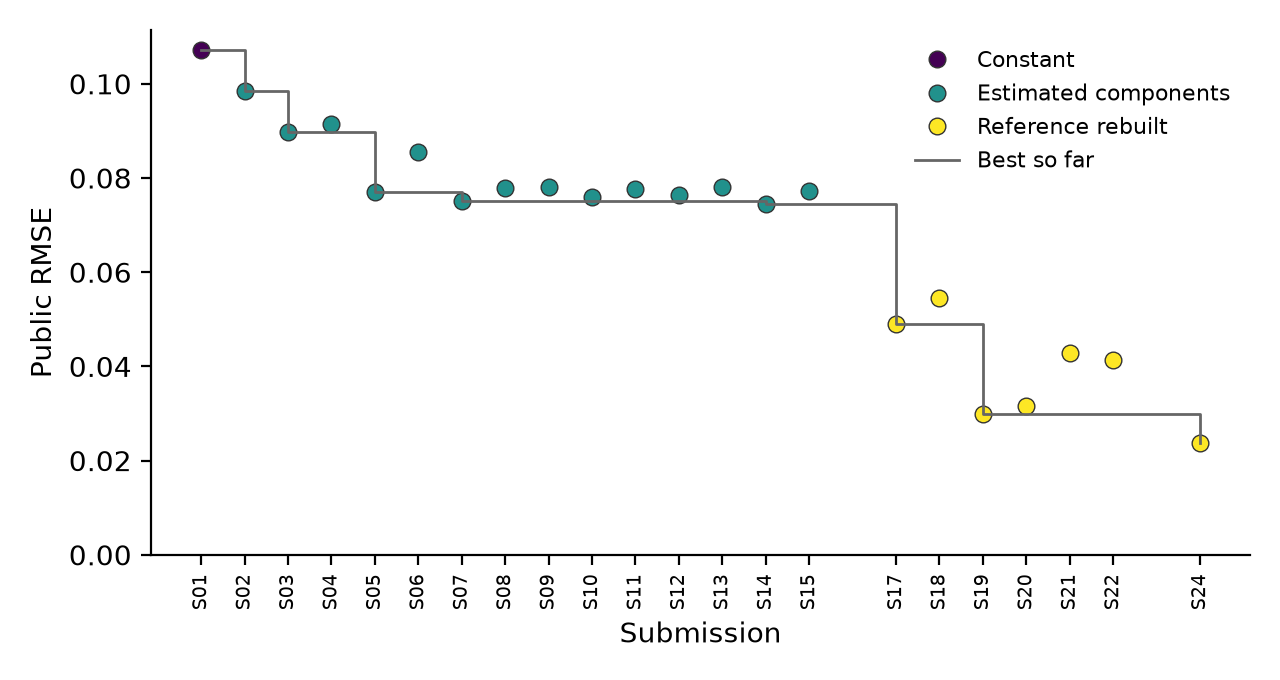
\includegraphics[width=0.85\textwidth]{fig_submissions.png}
\caption{Public RMSE by submission. S16 was not scored; S23, a competitor's
file uploaded as a benchmark, is left out.}
\label{fig:history}
\end{figure}

\begin{table}[htbp]
\centering
\small
\caption{Every scored submission, what it tested and what was decided.}
\label{tab:history}
\resizebox{\textwidth}{!}{%
\begin{tabular}{llrl}
\toprule
ID & Change tested & Public RMSE & Decision \\
\midrule
S01 & Sample submission, all zero & 0.10725 & Fixes $E[y^2]$ for later diagnostics \\
S02 & Analytic v1: route-network transport proxy, building and POI estimates & 0.09849 & Base \\
S03 & Boundary double counting of the transport reference, $d = 25$\,m & 0.08974 & Kept \\
S04 & Same with $d = 50$\,m & 0.09151 & 25\,m kept \\
S05 & POI as a regional constant & 0.07710 & POI variation carried little \\
S06 & Building reference from USFS building counts & 0.08545 & Dropped \\
S07 & Establishments half at 0 & 0.07518 & Kept \\
S08 & Lower transport reference noise & 0.07782 & Dropped \\
S09 & Tract-level facility half & 0.07805 & Dropped \\
S10 & Transport reference without ramps & 0.07590 & Dropped \\
S11 & Unclipped segment lengths & 0.07766 & Dropped \\
S12 & Transport level probe & 0.07632 & Scale 1.15 \\
S13 & Building level probe & 0.07801 & Baseline 0 \\
S14 & Combined levels & 0.07454 & Best estimate-only method \\
S15 & Fire stations drive the facility half & 0.07716 & Partly kept \\
S17 & Transport rebuilt from TIGER 2025 & 0.04906 & Kept \\
S18 & Building rebuilt from Microsoft US v2 & 0.05462 & Dropped \\
S19 & Fire and school gaps from USGS structures, $E = 0$ & 0.02996 & Final B \\
S20 & S19 with ZBP establishments apportioned by places & 0.03153 & Dropped \\
S21 & S19 with EMS from USGS ambulance services & 0.04289 & Dropped \\
S22 & S19 with HIFLD schools & 0.04136 & Dropped \\
S23 & A competitor's published file, uploaded as a benchmark & 0.00227 & Not ours \\
S24 & S19 with ZBP establishments apportioned by HUD business ratios & 0.02380 & Final A \\
\bottomrule
\end{tabular}}
\end{table}

\subsection{Reading a submission without labels}

Each public score fixes one inner product with the hidden target, and two
submissions together say how far to move from one towards the other. For a
current best $p$ and a candidate $q = p + d$ with public RMSEs $R_p$ and
$R_q$,
\begin{equation}
E[(y - p)\,d] = \tfrac{1}{2}\left(R_p^2 - R_q^2 + E[d^2]\right), \qquad
t^\ast = \frac{E[(y-p)\,d]}{E[d^2]},
\end{equation}
where $t^\ast$ is the step along $d$ that would minimise the error. A value
near 1 means the candidate's change is right in full, near 0 that it carries
no signal, and negative that it points the wrong way. This was used as a
diagnostic on whole-method pairs, to decide whether a hypothesis was right
(S19 from S17, $t^\ast = 0.93$), carried no signal (S22, 0.002) or pointed the
wrong way (S18, $-0.84$). No final submission is a fitted blend, and no
per-tract or per-region edit was ever driven by a score.

\subsection{Tuned scalars}

The project allowed at most six global scalars tuned on the public
leaderboard. Five were used during the estimation phase: the boundary
distance (25\,m from 0, 25, 50), the POI level (0.779), the transport value
scale (1.15), the building baseline gap (0 from 0.01 and 0.05) and the fire
model strength (0.3). The rebuilt method uses only the building baseline gap.

\subsection{Final selection}
\label{sec:final}

\begin{figure}[htbp]
\centering
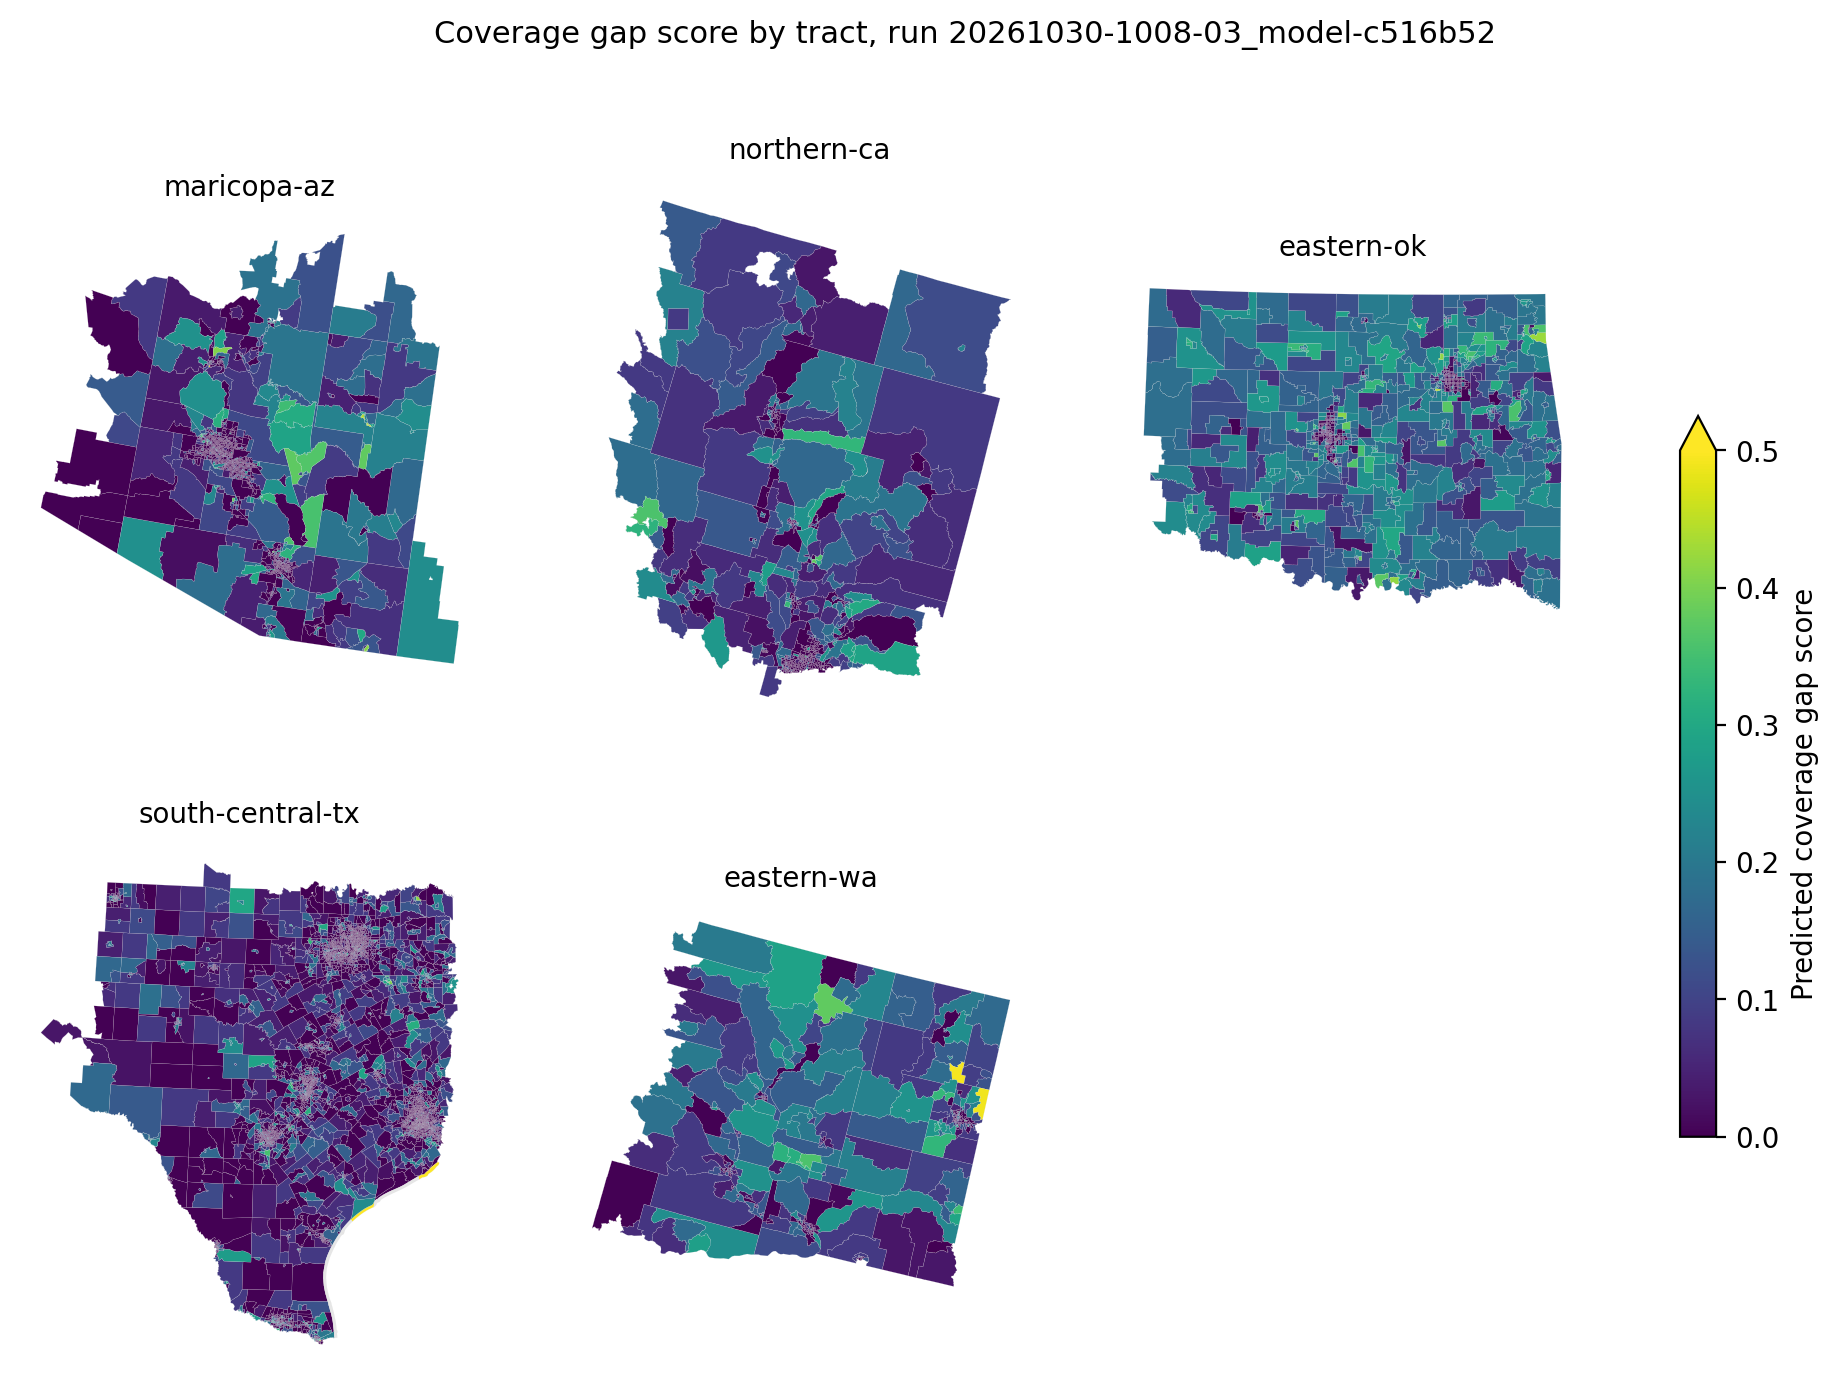
\includegraphics[width=\textwidth]{fig_map_scores.png}
\caption{S24 coverage gap score by tract, drawn by stage 04 from the S24
reproduction run. Scores above 0.5 share the top colour.}
\label{fig:map_scores}
\end{figure}

Figure~\ref{fig:map_scores} maps the S24 scores.

S24 is the best public score of this pipeline and depends on one tuned
scalar. S19 is the same method with the establishments half at 0. It differs
from S24 in 253 tracts and hedges the private split against the case where the
HUD apportionment fits the public tracts better than the private ones. S23 was
a competitor's published file, uploaded once to see its score. It was not
produced by this pipeline, its inputs include the organisers' removed
reference files, and it is not selected.

\section{Bias Scorecard reflections}
\label{sec:scorecard}

The scorecard reports disparity ratios of the predicted score between strata.
For the all-zero file every ratio was unavailable. Under the estimation phase
(S13) the tribal ratio was 1.30 and the rural ratio 1.25. On the scorecard for
S24 they are 2.92 for tribal against non-tribal tracts, 2.42 for rural against
urban, 1.22 for high social vulnerability, 1.46 for high climate
vulnerability and 1.81 for wildfire hazard, with summer heat the one stratum
where the gap is smaller (0.54). The rise comes
mostly from transport in Eastern Oklahoma, where 805 of 1,192 scored tracts
overlap a tribal area and the mean transport gap where defined is 0.355,
against 0.123 in South-Central Texas, and from fire stations, whose gap where
defined averages 0.44 in Eastern Oklahoma against 0.24 in Texas.

\section{Best Bias Discovery: unnamed local roads on tribal reservations}
\label{sec:bias}

\subsection{The pattern and why the scorecard cannot see it}

Every coverage measure in this challenge, and every metric on the Bias
Scorecard, counts length or features. A road segment that Overture holds
without a name adds as much length as a named one, so a tract whose roads
are all drawn but half unnamed scores as fully covered. The name is what
emergency services use. A caller gives an address, computer-aided dispatch
validates it against road centrelines that carry street names and address
ranges \cite{nena006}, and routing tools give instructions by street name.
This section shows that on federally recognised reservations a much larger
share of the local street network has no name in Overture than on comparable
non-tribal tracts, while the highways through the same reservations are
named as often as anywhere else.

\subsection{Measure and comparison}

For each scored tract the measure is the share of drivable road length
(Overture \texttt{roads} layer, classes motorway to unclassified, clipped to
the tract) whose \texttt{names.primary} is empty. It is computed separately
for the local classes (tertiary, residential, unclassified) and the named
classes (motorway, trunk, primary, secondary). Tracts are tribal when the
challenge's tribal overlap table links them to an American Indian, Alaska
Native or Native Hawaiian area, split into legal areas (reservations and
off-reservation trust land) and statistical areas (Oklahoma Tribal
Statistical Areas, OTSAs).

Rurality changes naming a great deal: in South-Central Texas the unnamed
share is 8\,\% in metropolitan tracts and 29\,\% in rural ones. Tribal tracts
are therefore compared with non-tribal tracts in the same region and RUCA
class (metropolitan, micropolitan, small town, rural), and the cell
differences are averaged with weights equal to the number of tribal tracts
in each cell. Intervals come from 1,000 bootstrap resamples of whole
counties, which keeps neighbouring tracts that share mapping history
together. All numbers come from stage 04 run
\texttt{20261030-1019-04\_analysis-8a838bb} on the challenge data only;
county names come from the Census 2020 county code list \cite{countycodes}.

\paragraph{Reproducing the finding.} Road length comes from
\nolinkurl{<region>-overture-roads.parquet} (classes motorway, trunk, primary,
secondary, tertiary, residential, unclassified), as geodesic metres of each
segment clipped to the tract polygons in \nolinkurl{<region>-census-tracts.parquet};
a segment is unnamed when \texttt{names.primary} is null. The tribal kind comes
from \nolinkurl{<region>-strata-tract-table.parquet}: a tract is a reservation
tract when \texttt{tribal\_legal} is true and a statistical-area tract when
\texttt{tribal\_any} is true and \texttt{tribal\_legal} is false; area names come
from \texttt{aiannh\_name} in \nolinkurl{<region>-tribal-tract-table.parquet}. The
rurality class maps \texttt{ruca\_primary} 1 to 3 to metropolitan, 4 to 6 to
micropolitan, 7 to 9 to small town and 10 to rural. Tracts with no drivable
road are left out, and tracts with no local road are left out of the local
comparison. In each region and class cell holding both groups, the mean
tribal share minus the mean non-tribal share is taken, and the cells are
averaged with weights equal to their tribal tract counts. The interval
resamples counties (the first five GEOID digits) with replacement 1,000
times and reports the 2.5th and 97.5th percentiles, dropping resamples in
which no cell holds both groups.

\subsection{Evidence}

Figure~\ref{fig:map_unnamed} maps the measure.
Table~\ref{tab:contrast} and Figure~\ref{fig:contrast} give the matched
differences. On the 80 reservation tracts, local streets are unnamed 9.5
percentage points more often than on matched non-tribal tracts (95\,\%
interval 3.5 to 14.7). The highways on the same tracts show no difference
($-0.4$, interval $-7.3$ to 5.6), so the gap sits on the streets where people
live and the measure is not picking up a regional habit of leaving highways
unnamed. The difference holds in each region with enough reservation tracts
to test: Maricopa (37 tracts, $+7.3$), Eastern Washington (16, $+4.5$) and
Eastern Oklahoma, where the Osage Reservation reaches $+27.6$ (9.8 to 29.6).
Northern California's 13 reservation tracts point the same way with an
interval that includes zero.

\begin{table}[htbp]
\centering
\small
\caption{Tribal minus non-tribal unnamed share of drivable length, matched
within region and RUCA class, in percentage points, with 95\,\% county
bootstrap intervals.}
\label{tab:contrast}
\begin{tabular}{llrrr}
\toprule
Tribal tracts & Roads & Tracts & Difference & Interval \\
\midrule
Reservations, all regions & local & 80 & $+9.5$ & 3.5 to 14.7 \\
Reservations, all regions & all drivable & 80 & $+8.3$ & 2.9 to 13.5 \\
Reservations, all regions & named classes & 79 & $-0.4$ & $-7.3$ to 5.6 \\
Osage Reservation, Eastern Oklahoma & local & 13 & $+27.6$ & 9.8 to 29.6 \\
Reservations, Maricopa & local & 37 & $+7.3$ & 3.0 to 10.9 \\
Reservations, Eastern Washington & local & 16 & $+4.5$ & 0.0 to 14.8 \\
Reservations, Northern California & local & 13 & $+3.8$ & $-2.9$ to 10.1 \\
OTSAs, Eastern Oklahoma & local & 792 & $+3.0$ & $-6.0$ to 7.5 \\
\bottomrule
\end{tabular}
\end{table}

\begin{figure}[htbp]
\centering
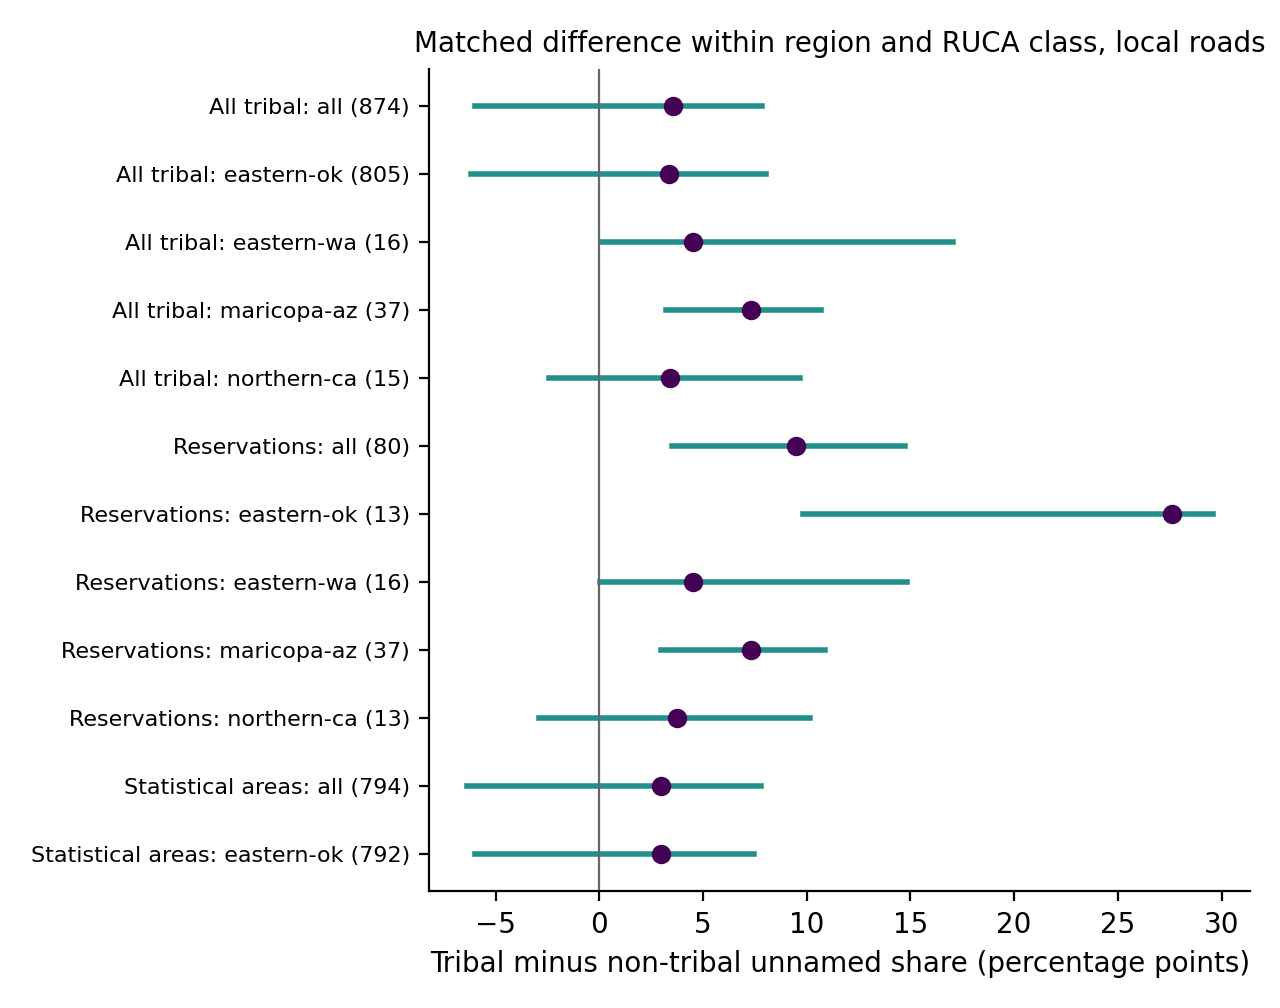
\includegraphics[width=0.68\textwidth]{fig_contrast_local.png}
\caption{Matched difference in the unnamed share of local street length,
tribal minus non-tribal tracts, with 95\,\% county bootstrap intervals.
Numbers in brackets are tribal tracts.}
\label{fig:contrast}
\end{figure}

\begin{figure}[htbp]
\centering
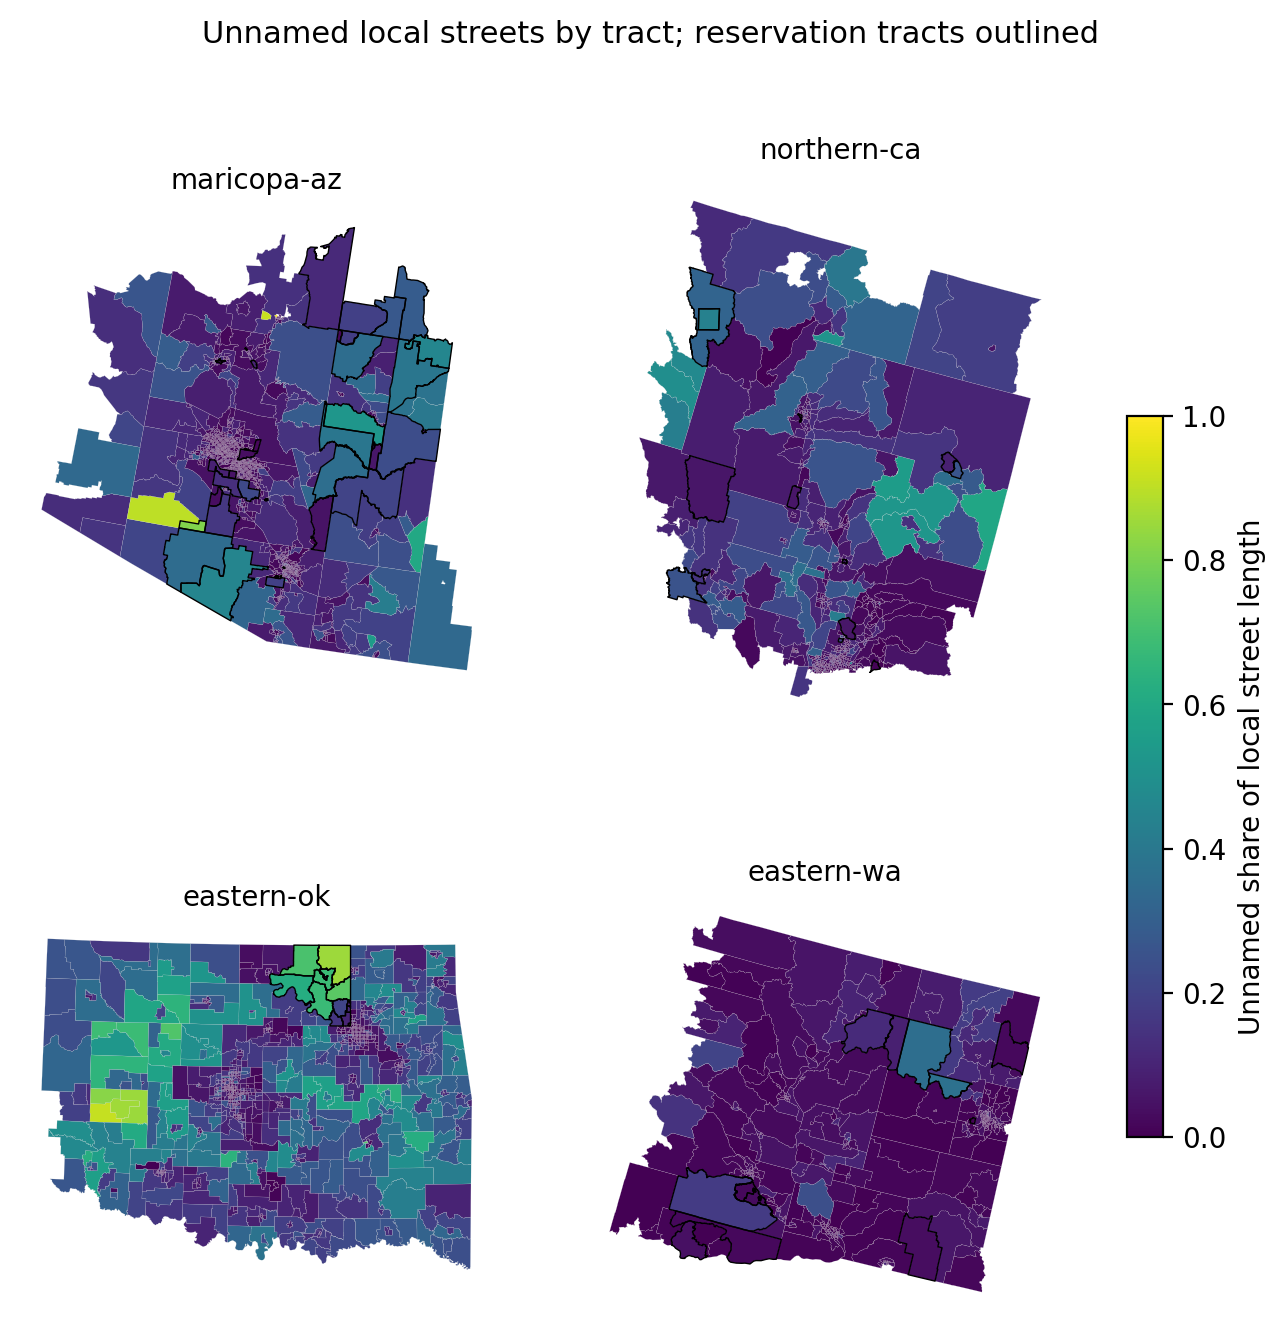
\includegraphics[width=0.85\textwidth]{fig_map_unnamed.png}
\caption{Unnamed share of local street length by tract (Overture
2026-08-19.0). Reservation tracts are outlined in black; the Osage Reservation
is the outlined block in north-central Oklahoma. Oklahoma Tribal Statistical
Areas are not outlined. Grey tracts have no local road.}
\label{fig:map_unnamed}
\end{figure}

The OTSAs hold the largest unnamed networks in absolute terms: 13,066\,km of
unnamed drivable road in the Cheyenne and Arapaho OTSA (47\,\% of its
network) and 8,831\,km in the Choctaw OTSA (34\,\%). After matching they do
not separate from non-tribal tracts, because 792 of Eastern Oklahoma's 1,192
scored tracts lie in an OTSA and only 43 non-tribal tracts outside its
metropolitan areas remain to compare with. The OTSA result is therefore
unresolved by this design, and the claim made here is limited to
reservations.

The 80 reservation tracts hold 294,612 residents and 8,266\,km of unnamed
drivable road. In 19 of them, home to 55,092 people, at least 30\,\% of local
street length has no name. That is 24\,\% of reservation tracts, against
13\,\% of non-tribal tracts once those are weighted to the same mix of
rurality.

Table~\ref{tab:tracts} names the reservation tracts with the most unnamed
road, with their wildfire history and social vulnerability from the
challenge's strata tables. Several of them combine a largely unnamed street
network with recent fire and high vulnerability. Tract 9400.04 in Osage
County, Oklahoma has 78\,\% of its drivable length unnamed and 29\,\% of its
land burned between 2015 and 2023. Tract 9400 in Ferry County, Washington,
on the Colville Reservation, has 498\,km of unnamed road, 27\,\% of its land
burned since 2015 and an SVI percentile of 0.84. Tracts 9408 and 9411 in
Pima County, Arizona, on the Tohono O'odham Nation Reservation in the
Sonoran Desert, have SVI percentiles of 0.96 and a third or more of local
street length unnamed.

\begin{table}[htbp]
\centering
\small
\caption{Reservation tracts with the most unnamed drivable road. Local:
unnamed share of local street length. Burned: share of land burned
2015 to 2023 (MTBS). SVI: CDC SVI 2022 overall percentile.}
\label{tab:tracts}
\resizebox{\textwidth}{!}{%
\begin{tabular}{llllrrrrr}
\toprule
GEOID & Tract & County & Reservation & Unnamed km & All & Local & Burned & SVI \\
\midrule
40113940004 & 9400.04 & Osage, OK & Osage & 606 & 0.78 & 0.86 & 0.29 & 0.48 \\
40113940003 & 9400.03 & Osage, OK & Osage & 524 & 0.62 & 0.62 & 0.12 & 0.74 \\
53019940000 & 9400 & Ferry, WA & Colville & 498 & 0.34 & 0.36 & 0.27 & 0.84 \\
04001970202 & 9702.02 & Apache, AZ & Zuni & 462 & 0.35 & 0.39 & 0.00 & 0.54 \\
40113940011 & 9400.11 & Osage, OK & Osage & 454 & 0.74 & 0.71 & 0.12 & 0.58 \\
06023010102 & 101.02 & Humboldt, CA & Yurok & 387 & 0.32 & 0.32 & 0.20 & 0.61 \\
04001970502 & 9705.02 & Apache, AZ & Fort Apache & 385 & 0.23 & 0.23 & 0.02 & 0.66 \\
04019940800 & 9408 & Pima, AZ & Tohono O'odham & 384 & 0.40 & 0.45 & 0.03 & 0.96 \\
40113940001 & 9400.01 & Osage, OK & Osage & 327 & 0.61 & 0.68 & 0.37 & 0.83 \\
04017940100 & 9401 & Navajo, AZ & Fort Apache & 324 & 0.47 & 0.52 & 0.07 & 0.87 \\
\bottomrule
\end{tabular}}
\end{table}

\subsection{Consequences}

\paragraph{Emergency dispatch.} An address on a road with no name in the map
cannot be matched to a centreline, so a 911 call from it geocodes to a
nearby named road, a ZIP centroid or nothing. On a reservation, response is
often shared between tribal, county, state and federal agencies, and units
arriving from outside lack the local knowledge that substitutes for a street
name. On the Osage Reservation, where 57\,\% of the drivable length has no
name and single tracts reach 78\,\%, a crew from a neighbouring county
routed by a tool built on open map data receives instructions in which most
turns are onto an unnamed road.

\paragraph{Evacuation routing.} Wildfire evacuation orders name the roads
to leave by and the zones they bound. Where a third of the local network is
unnamed, as on the Colville and Yurok tracts with a fifth to a quarter of
their land burned since 2015, zone maps and routing products drawn from open
data cannot describe the egress routes that residents of those roads would
need.

\paragraph{Disaster relief.} Damage assessment, supply distribution and
welfare checks during extreme heat, which the Tohono O'odham tracts face each
summer, are organised by address. Households on unnamed roads drop out of
address-based lists and have to be found by coordinates.

\paragraph{Why the scorecard misses it.} The Road Network Equity Ratio and
the other scorecard metrics compare lengths and counts, and the transport
component itself compares only motorway to secondary length. A reservation
whose streets are drawn but unnamed has full road coverage by every one of
these measures. The disparity becomes visible only through an attribute,
the name, that none of them reads.

\section{Limitations}
\label{sec:limits}

The gap form in Equation~\ref{eq:gap} is taken from the organisers'
description and README; their code was not available. The establishments
apportionment is undocumented; the HUD business-address ratios fit it well
($t^\ast = 1.17$), but the organisers' crosswalk quarter and Business
Patterns year are unknown. The organisers' Microsoft footprint release is unknown, and
the public release made the score worse, so the building component is held
at 0 where Overture has footprints. The TIGER 2025 and USGS 2026 files may
differ from the vintages the organisers used, and their EMS reference could
not be rebuilt from public data. The remaining public error of 0.024 sits in
these components. The bias discovery uses Overture names as
published. A road may carry a name in a local addressing system that
Overture does not hold; in that case the open map lacks the name, which is
the gap being measured.

\section*{Reproducibility statement}

Code, configuration and logs are in a private git repository that will be
released to Zindi reviewers on request. Every compute stage runs on Kaggle
from a code dataset built from a clean commit, with the commit hash written to
each output. The final submissions come from commits \texttt{30d804e} (S24)
and \texttt{672866c} (S19) with the overrides in Table~\ref{tab:overrides}.
Python 3.13.15 on the Kaggle image, DuckDB 1.5.4, numpy 2.1.3, pandas 2.3.3;
the full \texttt{pip freeze} is saved with each run. The seed is 20261025 for
every random generator. The rebuilt components involve no random draws. Both
final configurations were rerun on Kaggle from later code with
\texttt{make reproduce}: S19 on 29 October (run
\texttt{20261029-2244-03\_model-50be6bb}) and S24 on 30 October (run
\texttt{20261030-1008-03\_model-c516b52}). Each output matched the uploaded
file in every cell, with a largest float difference of 0 and no differing
flag. Runtimes and
memory are in Table~\ref{tab:stages}. The commands are
\texttt{make kaggle-run STAGE=<stage> SET="<overrides>"} for each stage in
the order 01, 02, 05, 06, 07, 03.

\begin{table}[htbp]
\centering
\small
\caption{Configuration overrides for the final submissions.}
\label{tab:overrides}
\begin{tabular}{ll}
\toprule
Submission & Overrides on \texttt{configs/model.yaml} \\
\midrule
S24 & \texttt{transport.source=tiger building.baseline\_gap=0 poi.source=reference} \\
    & \texttt{poi.reference\_types=[fire,schools] poi.establishment\_weight=bus} \\
S19 & as S24 with \texttt{poi.establishment\_weight=none} \\
\bottomrule
\end{tabular}
\end{table}

\begin{thebibliography}{99}

\bibitem{bucket}
Humane Intelligence (2026). Bias Bounty Mapping Equity Challenge data
repository and README. Source Cooperative.
\url{https://source.coop/humane-intelligence/bias-bounty-mapping-equity-challenge}

\bibitem{zindi}
Zindi (2026). Bias Bounty Mapping Equity Challenge.
\url{https://zindi.africa/competitions/bias-bounty-mapping-equity-challenge}

\bibitem{overture}
Overture Maps Foundation (2026). Overture Maps release 2026-08-19.0 and
schema documentation. \url{https://docs.overturemaps.org/}

\bibitem{nena006}
National Emergency Number Association (2022). NENA Standard for NG9-1-1 GIS
Data Model, NENA-STA-006.2-2022.

\bibitem{tiger}
US Census Bureau (2025). TIGER/Line Shapefiles 2025: primary and secondary
roads. \url{https://www2.census.gov/geo/tiger/TIGER2025/PRISECROADS/}

\bibitem{usgs}
US Geological Survey (2026). The National Map, Structures: state
GeoPackages. \url{https://prd-tnm.s3.amazonaws.com/StagedProducts/Struct/GPKG/}

\bibitem{zbp}
US Census Bureau (2025). ZIP Code Business Patterns 2023, totals file.
\url{https://www2.census.gov/programs-surveys/cbp/datasets/2023/}

\bibitem{zcta}
US Census Bureau (2022). 2020 ZCTA to census tract relationship file.
\url{https://www2.census.gov/geo/docs/maps-data/data/rel2020/zcta520/}

\bibitem{hud}
US Department of Housing and Urban Development. HUD USPS ZIP Code
Crosswalk Files, ZIP-TRACT, fourth quarter 2024. Archived copy: DataLumos
project 219325, version V2, retrieved 29 October 2026.
\url{https://www.datalumos.org/datalumos/project/219325/version/V2/view}

\bibitem{msbuildings}
Microsoft (2020). US Building Footprints, version 2.
\url{https://github.com/microsoft/USBuildingFootprints}

\bibitem{svi}
Centers for Disease Control and Prevention and ATSDR (2024). CDC/ATSDR Social
Vulnerability Index 2022.

\bibitem{ruca}
USDA Economic Research Service (2025). Rural-Urban Commuting Area codes,
2020.

\bibitem{countycodes}
US Census Bureau. 2020 national county code list
(\texttt{national\_county2020.txt}). Retrieved 29 October 2026.
\url{https://www2.census.gov/geo/docs/reference/codes2020/national_county2020.txt}

\end{thebibliography}

\end{document}
